\section{Design del Database}

Il database ha il ruolo della memorizzazione dei dati persistenti riguardanti l'applicazione.


\subsection{Modello concettuale}

La progettazione concettuale serve a rappresentare in maniera semplificata la realtà che poi andrà a identificare il sistema, per rendere facilmente leggibile tale astrazione viene fatto uso del diagramma    entità-relazione dal significato rapido e intuitivo. Questo modello ha il compito di organizzare il mantenimento dei dati in maniera propedeutica al loro utilizzo successivo e pertanto sarà essenziale alla realizzazione effettiva di tale raccolta informativa. 
\\[1\baselineskip]
Il diagramma entità-relazione è formato dalle entità che entrano in gioco in SWIMv2 e dalle relazioni che intercorrono tra di esse; è un passo intermedio
verso la definizione delle tabelle del database del sistema e mette in evidenza in che modo le entità interagiscono tra di loro.

\begin{figure} [!hbp]
\centering
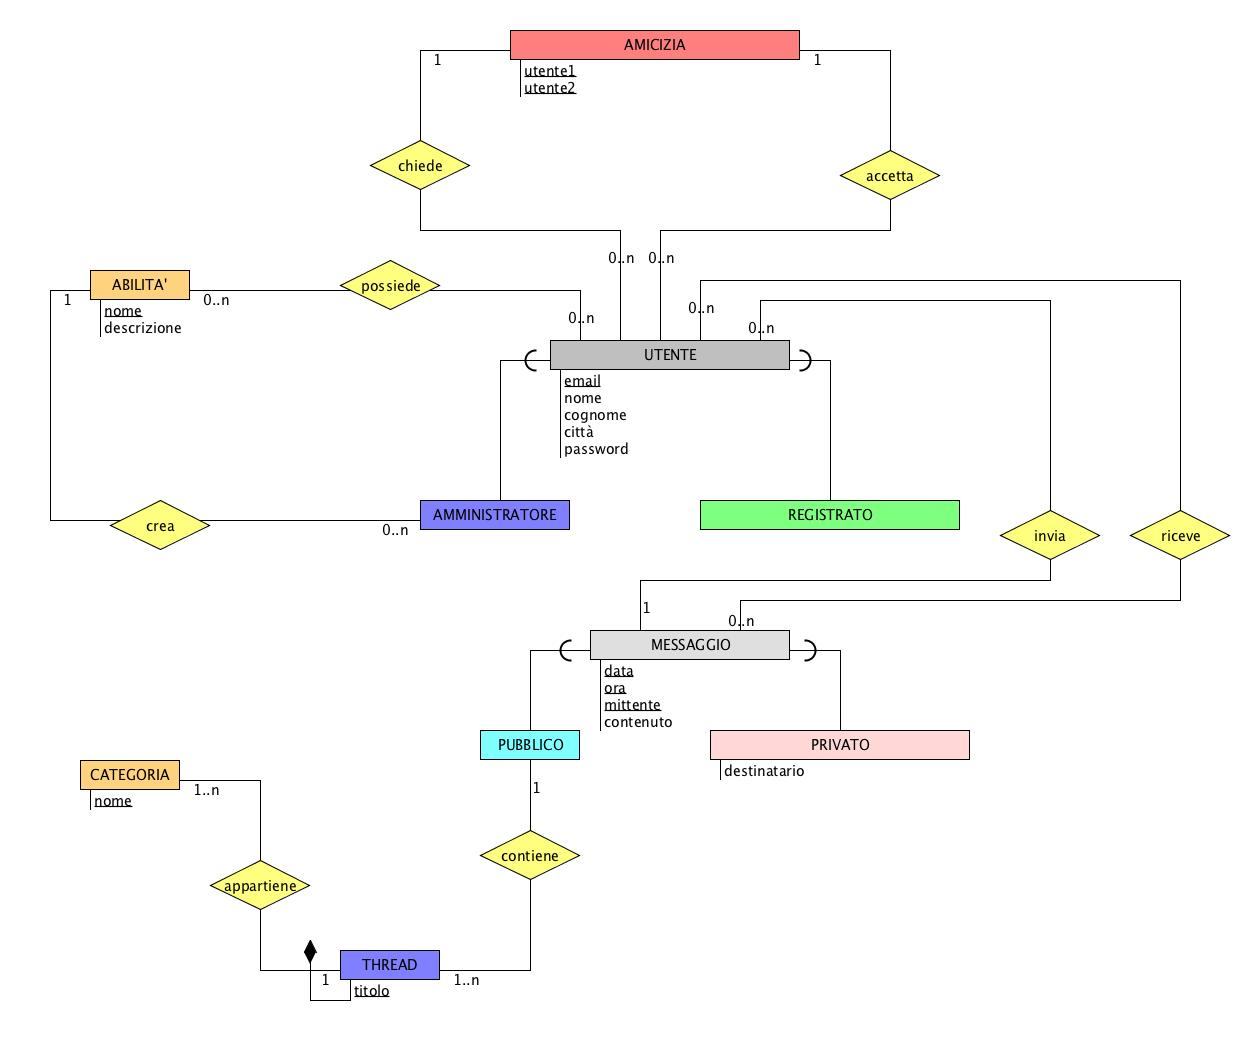
\includegraphics[scale=0.35]{ER.jpg} \\
\caption{\label{entitaRelazioni} Diagramma ER che sintetizza la struttura del database}
\end{figure}

\subsubsection{Entit\'a}
\begin{itemize}
 \item {\bfseries Utente}: è l'entità padre rappresentante un individuo autenticato in SWIM,  contenente quindi i dati di registrazione: nome, cognome,città, indirizzo email,password e un campo admin (ottenuto tramite un collasso verso l'alto della generalizzazione, nella tabella sarà di tipo boolean) che indica se l'utente è un amministratore.
 \item {\bfseries Amministratore}: è una delle due entità figlie di Utente che ha delle funzionalità in più riguardanti la gestione delle abilità.
 \item {\bfseries Registrato}: è l'altra entità figlia di Utente che ha le funzionalità dell'utente registrato a SWIM quali la richiesta di amicizia ad altri utenti e la replica ai messaggi.
 \item {\bfseries Messaggio}: è un'altra entità padre modella l'esistenza degli scambi testuali che avvengono tra gli utenti, ha come attributi la data, l'ora, il mittente e il contenuto.
\item {\bfseries Privato}: è un' entità figlia di Messaggio oltre a tutti gli attributi del padre è dotata anche del campo destinatario.
\item {\bfseries Pubblico}: questa entità si distingue dal Messaggio Privato poichè non ha il campo destinatario in quanto contenuta all'interno dei Thread.
\item {\bfseries Thread}: quando viene creata una discussione all'interno dell'applicazione nasce il Thread, esso è dotato di un titolo. 
\item {\bfseries Categorie}: rappresenta l'entità modellizzante gli argomenti principali di discussione all'interno del sistema 
\item {\bfseries Abilità}: è un' entità che rappresenta un modello delle capacità degli utenti, ha come attributi il nome e una breve descrizione. 
\item {\bfseries Amicizia}: l'entità rappresentante l'amicizia presente tra due utenti, ha come attributi le chiavi dei due amici.
\end{itemize}

\subsubsection{Relazioni}
\begin{itemize}
 \item {\bfseries chiede - accetta}: una delle funzionalità di SWIM permette all'utenza di richiedere e accettare richieste di amicizia tra di loro, questa relazione modellizza tale concetto.
 \item {\bfseries invia - riceve}: questa relazione indica la possibilità di inviare e ricevere messaggi di tipo pubblico e/o privato.
 \item {\bfseries possiede}: l'Utente possiede delle determinate abilità che caratterizzano il suo ruolo all'interno del Social Network.
 \item {\bfseries crea}: un Amministratore può creare delle nuove abilità che potrebbero anche essergli state suggerite da un Utente Registrato tramite messaggio privato.
 \item {\bfseries contiene}: un Thread contiene tutti i Messaggi Pubblici che lo riguardano.
 \item {\bfseries appartiene}: un Thread ha una Categoria di appartenenza che permette quindi di catalogare le varie argomentazioni trattate.
\end{itemize}

\subsection{Progetto Logico}

La progettazione logica ha il ruolo di trasformare il concetto espresso tramite il diagramma entità-relazioni in una descrizione logica della struttura dati. In questa fase l'ER prodotto precedentemente può subire delle variazioni necessarie a garantirne la funzionalità ed un' immediata traduzione in tabelle effettive all'interno del DBMS. 

\subsubsection{Ristrutturazione dello schema Entit\`a-Relazione}

\begin{itemize}
 \item[$\textcolor{red}{\diamondsuit}$]  La generalizzazione di Utente subisce un collasso verso l'alto, viene introdotto un attributo booleano "admin" che permetterà di differenziare l'attività dei due tipi diversi di utenti all'interno di SWIM.
 \item[$\textcolor{red}{\diamondsuit}$]  La generalizzazione Messaggio subisce un collasso verso il basso avremo quindi la tabella Messaggi Privati e la tabella Messaggi Pubblici.
\item[$\textcolor{red}{\diamondsuit}$] La relazione riceve-pubblici cessa di avere significato in quanto i Messaggi Pubblici sono associati ai Thread non ai singoli utenti, viene pertanto eliminata.
 \end{itemize}

\subsubsection{Traduzione verso il modello relazionale}

\begin{itemize}
\item[$\textcolor{red}{\diamondsuit}$] Le relazioni chiede-accetta 1 a molti si riassumono nel realizzare l'unica tabella Amicizia con le due chiavi degli utentiche essendo già presenti in tale relazione non devon esser aggiunte.
\item[$\textcolor{red}{\diamondsuit}$] La relazione possiede essendo una molti a molti va risolta creando una tabella apposita che ha come attributi chiave il nome dell'Abilità e l'email dell'Utente. 
\item[$\textcolor{red}{\diamondsuit}$] La relazione crea 1 a molti va trattata aggiungendo all'interno della tabella delle Abilità come attributo l' email-dell'amministratore che l'ha realizzata.
\item[$\textcolor{red}{\diamondsuit}$] La relazione appartiene 1 a molti con l'entità debole Thread si risolve aggiungendo all'interno della tabella Thread l'attributo nome-categoria come chiave.
\item[$\textcolor{red}{\diamondsuit}$] La relazione contiene 1 a molti viene trattata come crea ossia si aggiunge alla tabella Messaggio Pubblico l'attributo titolo-thread.
\item[$\textcolor{red}{\diamondsuit}$] La relazione riceve-privati essendo una molti a molti porta alla realizzazione di una tabella apposita contenente le chiavi del Messaggio Privato in quanto l'attributo mittente indica già la mail dell' Utente che ha mandato il messaggio.
\item[$\textcolor{red}{\diamondsuit}$] Le relazioni invia-privati e invia-pubblici essendo 1 a molti si sarebbero risolte aggiungendo alle tabelle dei due tipi di messaggi l'attributo email-mittente che siccome è già presente non necessitano di ulteriori modifiche.
 \end{itemize}

\clearpage

Le tabelle risultanti dalla traduzione del diagramma ER sono:
\begin{itemize}
\item[--]Utente(\underline{{\bfseries email}}, nome, cognome, città, password, admin);\\
\item[--]Amicizia(\underline{{\bfseries email-utente1}}, \underline{{\bfseries email-utente2}});\\
\item[--]Abilità(\underline{{\bfseries nome}}, email-amministratore, descrizione);\\
\item[--]Messaggio Pubblico(\underline{{\bfseries data}}, \underline{{\bfseries ora}}, \underline{{\bfseries mittente}}, titolo-thread, contenuto);\\
\item[--]Messaggio Privato(\underline{{\bfseries data}}, \underline{{\bfseries ora}}, \underline{{\bfseries mittente}}, destinatario, contenuto);\\
\item[--]Categorie(\underline{{\bfseries nome}});\\
\item[--]Thread(\underline{{\bfseries titolo}}, \underline{{\bfseries nome-categoria}} );\\
\item[--]Possiede-Abilità(\underline{{\bfseries email-utente}}, \underline{{\bfseries nome}});\\
\item[--]Riceve-Privati(\underline{{\bfseries email-mittente}}, \underline{{\bfseries data}}, \underline{{\bfseries ora}});
\end{itemize}

\begin{figure} 
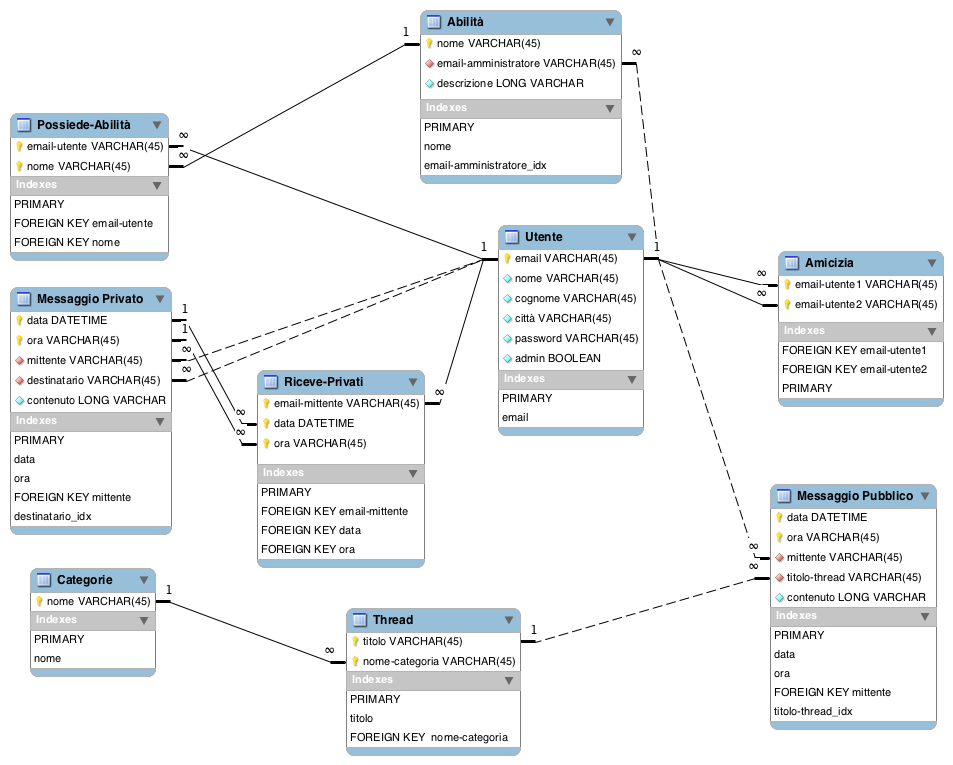
\includegraphics[scale=0.55]{GraficoRelazionale.png} \\
\caption{\label{RelazioniTabelle} Relazioni tra le tabelle nel database}
\end{figure}
